\chapter{Evaluation}

%123456789 123456789 123456789 123456789 123456789 123456789 123456789 123456789

\label{ch:evaluation}

In this chapter we aim to empirically evaluate the approaches we have described
in previous chapters of this work.

\section{Datasets}

\label{sec:datasets}

In this thesis we work with two distinct \glspl{ses}.

The first \gls{ses} comes from processing recording from single camera which
capture a busy square. The original recording is about 5 minutes long. The total
number of \glspl{det} extracted from the recording is 181,792. We manually sorted
these \glspl{det} into 274 different \glspl{iden}. The main usage of this
\gls{det} is to be a training dataset for training neural network based
approaches to extract feature vectors from the images of \glspl{det}. The
manual annotation serves as a golden truth for this training. A frame from
this \gls{ses} and extracted \glspl{det} can be seen in
\autoref{fig:single_session}.

\begin{figure}
    \centering
    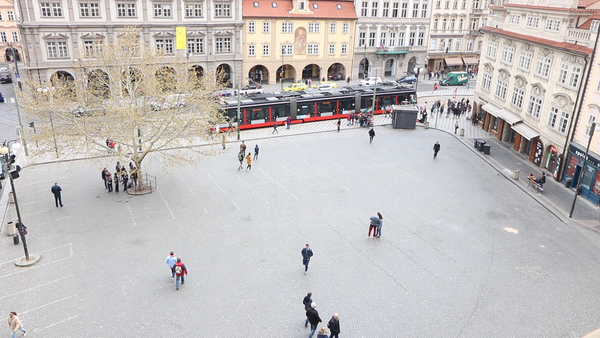
\includegraphics[width=0.48\textwidth]{img/frame_single_session_smaller.png}
    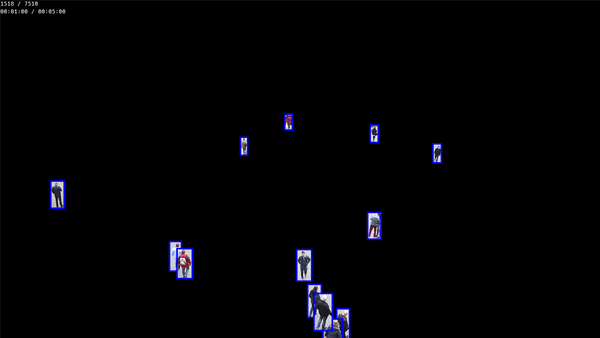
\includegraphics[width=0.48\textwidth]{img/frame_single_session_det_smaller.png}
    \caption{Frame from first session and extracted detections}
    \label{fig:single_session}
\end{figure}

We use the second \gls{ses} for actual evaluation. This second session is
constructed from the recording of two simultaneously recording camera. The
recording is over two minutes long. The view of the cameras partially overlap.
In this session total of 147,681 \glspl{det} were extracted. We sorted these
\glspl{det} into 52 unique \glspl{iden}. These \glspl{iden} were used as a
ground truth for actual evaluation of our approach. Examples of frames from
this \gls{ses} is in \autoref{fig:double_session}.

\begin{figure}
    \centering
    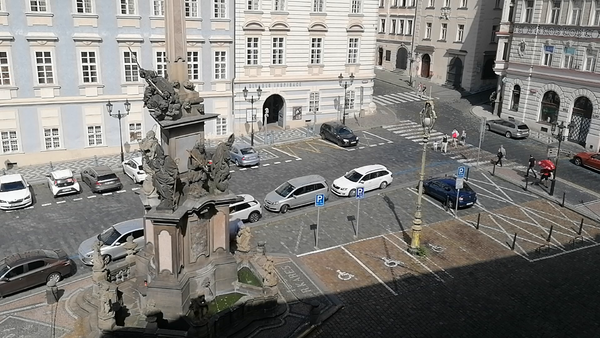
\includegraphics[width=0.48\textwidth]{img/frame_double_session_1_smaller.png}
    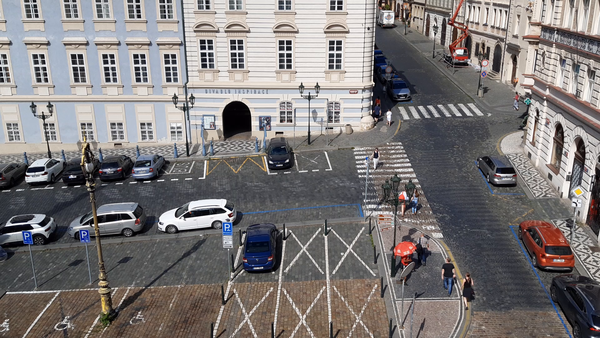
\includegraphics[width=0.48\textwidth]{img/frame_double_session_2_smaller.png}
    \caption{Frames from second session}
    \label{fig:double_session}
\end{figure}

The recordings for those two \glspl{ses} are entirely disconnected -- they
capture entirely different place and were recorded at different time. That gives
us unbiased estimation of the quality of our algorithm in terms of
\autoref{eq:mla}. It would be better to evaluate our algorithm to multiple
\glspl{ses}, however due to technical difficulty of creating new \gls{ses}
(especially in terms of annotating the data), we leave more thorough evaluation
to feature work.

\section{Feature vectors}

As the first step of actual evaluation of our approaches we evaluate the
quality of feature vectors as described in \autoref{ch:features}. We shall
evaluate this part purely based on how well the resulting feature vectors
separate the golden \glspl{iden} from each other. We recognize there is some
information lost, as we skip the final step in this evaluation -- that is to
construct actual \glspl{iden} and compare them with the golden \glspl{iden}.
However, this preliminary evaluation is computationally less expensive and
therefore we may experiment with broader spectrum of parameters. We shall
select couple of best performing setting and verify its usefulness in later
stages.

\subsection{Measures of Quality}

This preliminary testing offer simpler statistics for evaluation. In this scenario we need to just look into distances between \glspl{det} of the same golden \gls{iden} and the distances between \glspl{det} of distinct golden \glspl{iden}. We can further associate each approach with a threshold. The ideal scenario would be that the maximal distance between \glspl{det} from the same \gls{iden} would be at most this threshold and all the distances between \glspl{det} from distinct \glspl{iden} would be greater than the threshold. However, in most cases we do not have such ideal classifier. Thus we often need to deal with misclassified samples.

Overall we can assign every pair of detection in on of four standard categories. First two are \glspl{tp} and \glspl{tn} they represent correct classification -- pair of \glspl{det} from the same \gls{iden} with distance between them below selected threshold and pair of \glspl{det} from distinct \glspl{iden} with distance over the threshold respectively. The other categories are \glspl{fp} -- pairs that are of different \glspl{iden} but with distance below the threshold -- and \glspl{fn}, that are pairs of \glspl{det} from the same \gls{iden} but with the distance over the threshold.

This notation allows us to introduce two standard derived quantities --- \gls{tpr} and \gls{fpr}:

\begin{align*}
    \mathrm{TPR} &= \frac{\mathrm{TP}}{\mathrm{TP} + \mathrm{FN}} \\
    \mathrm{FPR} &= \frac{\mathrm{FP}}{\mathrm{FP} + \mathrm{TN}}
\end{align*}

Notice that when we increase the threshold, increase the number \glspl{tp} and \glspl{fp} and decrease number of \glspl{tn} and \glspl{fn}. In terms of rates, that means that both \gls{tpr} and \gls{fpr} increases. This allows us to draw a plot of how \gls{tpr} depends on \gls{fpr}. That is a quite common way to elaborate on the quality of \gls{ml} algorithm. The resulting plot is often called \gls{roc} curve.

Ideal classifiers would have a \gls{roc} curve going through a point
(0, 1). Such classifier with corresponding threshold would correctly
classify every input, positive or negative. We usually do not
have access to ideal classifiers. In such case we are, broadly speaking,
want to come up with classifier that have \gls{roc} curve as close to
point (0,1) as possible.

However, \gls{roc} curves gives us more in-depth view into the classifier.
The curve shows which trade-offs between \glspl{fp} and \glspl{fn} (or in terms
of the axis \gls{fpr} and \gls{tpr}) are possible for given classifiers.

While the \gls{roc} curve offers quite useful evaluation of the
selected approach, it is often useful to express the quality of the
approach as a single number. Some information will be lost this way,
on the other hand it offers very straight-forward way to compare different
classifiers. For this evaluation we leverage also leverage the \gls{roc} curve.
In particular we compute the area under the curve. Generally, the greater
the area the better classifier we have.

Finally, let us note that we want to get feature vectors that help us to find the same object in physically distant \glspl{det}. Therefore, we are not really interested in the distance between \glspl{det} of the same \gls{iden} from subsequent frames (as they would be matched by metadata anyways without the visual information). Therefore, for this preliminary evaluation (and drawn \gls{roc} curves) out of all ``positive'' pairs (i.e. pairs of \glspl{det} from the same \gls{iden}) only those which are either from different cameras or are at least 2 seconds apart.

\subsection{Evaluation of Color Histograms}

Firstly, we aim to evaluate various approaches for feature vector generation
based on the color histograms. To recapitulate there are several basic choices
for histogram generation we need to evaluate (please refer to
\autoref{sec:histograms} for detailed explanation):

\begin{itemize}
    \item Selection of color model
    \item Type of background filtering
    \item Number of bins of a histogram
    \item Choice of distance function
\end{itemize}

\subsubsection{Evaluation of Background Filtering}

As there are too many options per category to evaluate all combinations we
firstly evaluate which background filtering mechanism works best for us. As we
aim to decide what section of the crop is important for the re-identification
the selection of background filtering should be relatively independent of
the choice of color model and number of bins. For the experiments in this
subsection we selected a hue and saturation with histogram with 8 bins in
each component (i.e. 64 bins total).

Let us recall that we reviewed several approaches to background filtering.
Each approach allows for fine-tuning via various parameters:

\begin{itemize}
    \item No background filtering -- no additional parameters
    \item Filtering using cropping -- total of three parameters: percentage of the image cropped from left and right, percentage of the image cropped from the bottom, and percentage of the image cropped from the top
    \item Weighting by Gaussian -- total of two parameters: center of the Gaussian along $y$-axis and the scale of the Gaussian
\end{itemize}

For each of these approaches we use grid search to find optimal values of
these parameters. The main value we use for comparison is the size of the
area under the \gls{roc} curve. However, we still explore some of the
\gls{roc} curves directly.

\begin{figure}
    \centering
    \def\svgwidth{\columnwidth}
    \Large
    \scalebox{0.6}{\input{img/aoc_crop_30.pdf_tex}}
    \scalebox{0.6}{\input{img/aoc_crop_20.pdf_tex}}
    \scalebox{0.6}{\input{img/aoc_crop_40.pdf_tex}}
    \caption{Area under the ROC curve for various copping setting}
    \label{fig:aoc_crop}
\end{figure}

As we can see from the measurements in \autoref{fig:aoc_crop} any method of background filtering significantly improved the quality of the feature vectors. We note that we achieved the best performance with cropping when we 
cropped 30\% image from the left and right side, 20\% from the top and 30\%
from the bottom (although variant with 20\% achieved almost as good results). An example of such cropping can be seen in
\autoref{fig:best_cropping}.

\begin{figure}
    \centering
    
\includegraphics{img/0.png} 
\includegraphics{img/1.png} \\
    
\includegraphics{img/0_crop.png} 
\includegraphics{img/1_crop.png}
    \caption{Example of most effective cropping}
    \label{fig:best_cropping}
\end{figure}

\begin{figure}
    \centering
    \def\svgwidth{\columnwidth}
    \Large
    \scalebox{0.6}{\input{img/aoc_gauss.pdf_tex}}
    \caption{Area under the ROC curve for various setting of Gaussian weighting}
    \label{fig:aoc_gauss}
\end{figure}

In terms of weighting with Gaussian, we have achieved the best results
by offsetting the Gaussian slightly above the center of the image, to 40\%
of the height of the image to be precise. The best setting for the scale
of the Gaussian seems to be 0.2 or 0.1 of the dimensions of the image. For detailed results
of the grid search see \autoref{fig:aoc_gauss}.

As we can see in \autoref{fig:roc_background} all the selected approaches
with background filtering gives almost identical results.

\begin{figure}[tb]
    \centering
    \def\svgwidth{\columnwidth}
    \input{img/background_roc.pdf_tex}
    \caption{ROC curve of various type of background filtering}
    \label{fig:roc_background}
\end{figure}

\subsubsection{Choice of distance function}

Another subject of our experiments is the choice of distance function. In
\autoref{ssec:used_distances} we introduced three distance functions --
Euclidean, Manhattan and cosine. As we can see in \autoref{fig:roc_distances}
the choice of distance function have significant effect on the results.
The worst distance function seems to be Euclidean distance. The best one,
especially while preserving lower \gls{fpr} seem to be Manhattan distance.
After all, Manhattan distance has quite straigh-forward explanation in context
of histograms -- it is simple the amount each bin needs to decrease or increase
in order to achieve the second histogram.

\begin{figure}
    \centering
    \def\svgwidth{\columnwidth}
    \input{img/roc_distances.pdf_tex}
    \caption{ROC curve of various distance functions}
    \label{fig:roc_distances}
\end{figure}

\subsubsection{Selection of Color Model and Number of Bins}

The last parameter we need to appropriately set is the actual color model
and number of bins per histogram. We explore several color models:

\begin{itemize}
    \item RGB model
    \item HSV model (we select hue component for one histogram and both hue and saturation component for another one)
    \item YUV model (we select UV components)
\end{itemize}

\begin{figure}
    \centering
    \def\svgwidth{\columnwidth}
    \Large
    \scalebox{0.7}{\input{img/model_bins.pdf_tex}}
    \caption[Area under the ROC curve for various color models and number of bins]{Area under the \gls{roc} curve for various color models and number of bins. Number of bins are displayer per channel. Total number of bins for HS and UV is number of bins per channel squared and for RGB it is number of bins per channel cubed. For some combinations were not explored as a total number of bins for these combination requires too much memory stored per each feature vector.}
    \label{fig:model_bins}
\end{figure}

For each model we explore various numbers of bins. The sizes of areas under the corresponding \gls{roc} curves is displayed in \autoref{fig:model_bins}. Contrary to our original
assumption the results gives usage of the raw RGB channels. The best variation in particular was with 4 bins per channel (i.e. 64 bins total).

This can be explained by various phenomena For one the varying lightning
conditions are not as common in our dataset as we expected. The other aspect
is that as we notice large quantity of the images are of people with black or
dark clothing. The downside of using hue as a component in histograms is that
hue can change very significantly case of black and white colors even in small
changes in actual color. See \autoref{fig:bad_hue} for the visualization.

\begin{figure}
    \centering
    
\includegraphics[width=3cm]{img/bad_hue_orig.png}
    
\includegraphics[width=3cm]{img/bad_hue_hue.png}
    \caption[Hue extraction from an image]{Hue extraction from an image. The image on the left is original. The right image was obtained by preserving hue of each pixel but setting saturation and value to the same high level. As we can see, the mono-colored black coat has various hue levels and on the other hand the black coat and the white background is represented by similar hue levels even tough both are of entirely different colors.}
    \label{fig:bad_hue}
\end{figure}

We aim to support this reasoning by considering pixels with low ($< 0.2$)
value as black and non-black pixels with low saturation ($< 0.2$) as white and
assign them to separate bins. As we can see in \autoref{fig:black_white_roc} this indeed
significantly improved the feature vector. However it still seems best to use basic RGB decomposition.

\begin{figure}
    \centering
    \def\svgwidth{\columnwidth}
    \input{img/black_white_roc.pdf_tex}
    \caption[Effect of adding black and white bins to hue histograms]{Effect of adding black and white bins to hue histograms. The figure shows \gls{roc} curves of histogram based approaches of with RGB, hue \& saturation and only hue decomposition with the best performing number of bins in each category. The plot shows improved performance obtained by adding black and white bins to the latter two categories.}
    \label{fig:black_white_roc}
\end{figure}

\subsection{Evaluation of Deep Learning Approaches}

In the previous section we have focused on the feature vectors drawn using
histograms. Now, we explore the approaches involving \glspl{nn}. In this
section we make use of pre-trained model in Tensorflow framework
(\cite{tensorflow}) and described in \autoref{sec:existing_architectures}.

\subsubsection{Direct Use of Pre-trained Models}

Perhaps the simplest usage of pre-trained models is to use them directly
wihtout any additional training. The potential in such usage is that the
second to last layer (i.e. prior actual ``classification'' layer) has to
contain enough of information to classify the original image. Therefore,
we experiment whether such information is enough for our purposes.

As we already stated, we mainly use ResNet and MobileNet architectures
pre-trained on the ImageNet dataset. These archtecture, as is common,
requires the input of the fixed size. That means we need to rescale all the
input images. As the sizes of original bounding boxes are diverse (see
\autoref{fig:size_dist}, we can not avoid distorting the original images.
Therefore, we evaluate performance of the network with various input sizes.

\begin{figure}
    \centering
    \def\svgwidth{\columnwidth}
    \input{img/size_distribution.pdf_tex}
    \caption{Distribution of heights and widths of detections}
    \label{fig:size_dist}
\end{figure}

The \gls{roc} curves (with the same setting as in previous subsection) of the
annotation with the pre-trained models in \autoref{fig:pretrained_nn_roc}.
We have evaluated various input sizes. In case of MobileNet we have tested
all the input sizes that are available for the architecture. As for the 
ResNet we have tested lower number of smaller sizes, mainly for its higher
complexity and poorer performace compared to the MobileNet.

As we can see directly from the \gls{roc} curves, the decidedly best setting for this type of the \gls{nn} annotation is MobileNet with input resized to $128 \times 128$. 

\begin{figure}
    \centering
    \def\svgwidth{\columnwidth}
    \input{img/pretrained_nn_roc.pdf_tex}
    \caption{ROC curves of pre-trained model}
    \label{fig:pretrained_nn_roc}
\end{figure}

We have also experimented with different distance functions. As you can in \autoref{fig:basic_nn_roc_dist} the effect of different distance functions are rather small. Especially between Euclidean and Manhattan distance.

\begin{figure}
    \centering
    \def\svgwidth{\columnwidth}
    \input{img/basic_nn_roc_dist.pdf_tex}
    \caption{Comparison of effect of different distance functions on MobileNet with shape 128}
    \label{fig:basic_nn_roc_dist}
\end{figure}

\subsubsection{Fine-tuning the Pre-trained Models}

As we showed we achieved somewhat useful results with just using as-is pre-trained models. However such models were trained for classification tasks and therefore there should be a room for improvement when trained specifically on \reid{} task. For this reason we aim to train the networks (with weights initialized as trained on classification task) on our dataset.

For the first experiment in this regard we do not change the architecture at all. We just use the architecture as-is and train in on our dataset using Triplet Loss (\autoref{sec:triplet_loss}).

\begin{figure}
    \centering
    \def\svgwidth{\columnwidth}
    \large
    \scalebox{0.8}{\input{img/training_loss.pdf_tex}}
    \caption{Training loss during training}
    \label{fig:training_loss}
\end{figure}

As we can see from the log in \autoref{fig:training_loss} we significantly reduce the training error by this approach. However when we tried to apply the resulting \gls{nn} on our testing \gls{ses} (see \gls{roc} curve in \autoref{fig:basic_nn_overfit_roc}), we see that the performance of the network significantly decreased. Furthermore, we can see that the performance worsen even after the single epoch of training. The weights are being altered too much even in single epoch as the original capabilities of the network is lost.

\begin{figure}
    \centering
    \def\svgwidth{\columnwidth}
    \input{img/basic_nn_overfit_roc.pdf_tex}
    \caption{Performance of the network after training for several epochs}
    \label{fig:basic_nn_overfit_roc}
\end{figure}

We therefore lowered the learning rate to try to preserve the original information within the network. This proved to be the correct approach as we manage to significantly increase the performance of the network as you can see in \autoref{fig:basic_nn_lr1_roc} and \autoref{fig:basic_nn_lr2_roc}.

\begin{figure}
    \centering
    \def\svgwidth{\columnwidth}
    \input{img/basic_nn_lr1_roc.pdf_tex}
    \caption{Performance of the network after training with learning rate 0.0001}
    \label{fig:basic_nn_lr1_roc}
\end{figure}

\begin{figure}
    \centering
    \def\svgwidth{\columnwidth}
    \input{img/basic_nn_lr2_roc.pdf_tex}
    \caption{Performance of the network after training with learning rate 0.00002}
    \label{fig:basic_nn_lr2_roc}
\end{figure}

Now, we proceed evaluate effect of different distance functions. This also means to train a new \gls{nn} as used loss function (Triplet Loss -- \autoref{eq:triplet}) depends on the choice of the distance function. In other related work we see the Triplet Loss used either with Euclidean distance or Cosine distance (or alternatively squared Euclidean distance\footnote{As the final layer of our \glspl{nn} is normalizing layer, the square Euclidean distance and cosine distance are proportional to each other: $\delta_{euclid}(\vec{x}, \vec{y}) = 2 - 2\vec{x}^T\vec{y} = 2 - 2 \cos(\vec{x}, \vec{y})$ (as the norms of input vectors are 1).}). However, we also aim to verify usefulness of Manhattan distance, as it works well with the histogram approach.

As you can see in \todo{ref}, the with different distance functions (both cosine and Manhattan) we achieved better results. As we can see in detailed 

